\chapter{Background}
\label{chap:background}
% Explain what this chapter is all about!
In this chapter we will give an introduction to background for our master thesis as well as the tools, technology and previous research that made it all possible. 

\section{Concepts}
    % Chapter intro outlining Our background and general motivation
    This section will take a look at the background for our project. What ideas laid the foundation for our motivations into this field.
    
    \subsection{Virtuality Continuum}
    The Virtuality Continuum(VC), as shown in Figure \ref{fig:virtualcontinuum}. "Is a concept which relates the mixture of classes of objects presented in any particular display situation."\cite{Milgram1994} This article, "\emph{A Taxonomy of Mixed Reality Visual Displays}" by Paul Milgram and Fumio Kishino\cite{Milgram1994} introduces the concept of a "virtuality continuum" to describe the range of environments shown on any particular display. The articles focus on the taxonomy of Mixed Reality displays, and is also one of the earliest adapters of the concept of Mixed Reality.
    \begin{figure}[!ht]
        \centering
        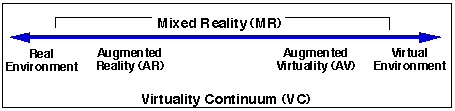
\includegraphics[scale=1]{figures/virtualcontinuum.png}
        \caption{Simplified representation of a "virtuality continuum".\cite{Milgram1994}}
        \label{fig:virtualcontinuum}
    \end{figure}
    
    \subsubsection{Virtual Reality}
    Using Milgram's and Kishinos's description of Virtual Reality(VR) from their paper.\cite{Milgram1994} VR is the concept of a virtual space where the user is fully immersed in a virtual world, usually through a Head Mounted Display(HMD). This means that the environment, and everything the user sees and interacts with is completely synthetic. The environment can emulate the real world and seem like reality, be it fiction or otherwise; or this virtual environment might be a world where our physical laws do not apply. On the virtuality continuum, as shown in Figure \ref{fig:virtualcontinuum}, this type of environment resides on the furthest extreme, opposite the real environment.

    \subsubsection{Augmented Reality}
    Augmented Reality(AR) is the concept of a real environment with digital elements superimposed, enhancing the users perception of reality.This is achieved by rendering these digital "\emph{holograms}" on a transparent display which the user sees through(e.g. Microsoft's Hololens or Magic Leap. The same effect can also be achieved by superimposing the digital elements onto video captured by a camera in real-time.
    
    \subsubsection{Mixed Reality}
    As shown in Figure \ref{fig:virtualcontinuum}, a Mixed Reality(MR) display can reside anywhere between the extremes of the virtuality continuum\cite{Milgram1994}. The technology has moved on since 1994, when the paper by Kishino and Milgram was published. \emph{"Since then, the application of mixed reality goes beyond displays but also includes environmental input, spatial sound, and location."}\cite{wdc-mr}
    
    Microsoft, especially, has expanded on the application of Mixed Reality. And in the article "What is mixed reality?"\cite{wdc-mr}. MR is described like this: \emph{"Most mobile phones on the market today have little to no environmental understanding capabilities. Thus the experiences they offer cannot mix between physical and digital realities. The experiences that overlay graphics on video streams of the physical world are augmented reality, and the experiences that occlude your view to present a digital experience are virtual reality. As you can see, the experiences enabled between these two extremes is mixed reality"}\cite{wdc-mr}. This spectrum is found in Figure \ref{fig:mrspectrum}
    
    \begin{figure}[!ht]
        \centering
        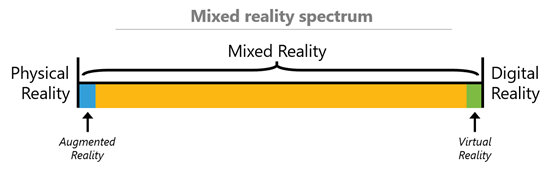
\includegraphics[scale=1]{figures/mixedrealityspectrum.png}
        \caption{The Mixed Reality Spectrum\cite{wdc-mr}}
        \label{fig:mrspectrum}
    \end{figure}
    
    In Figure \ref{fig:mrdevicetypes} the two main device types that deliver Windows Mixed Reality is listed. These are: Holographic devices, which has the ability to place digital content in the real world;\cite{wdc-mr} and Immersive devices, which has the ability to hide the physical world and replace it with a digital experience.\cite{wdc-mr} 
    \begin{figure}[!ht]
        \centering
        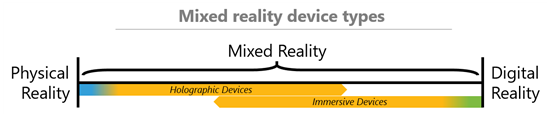
\includegraphics[scale=1]{figures/mixedrealityspectrumdevicetypes.png}
        \caption{Mixed reality device types.\cite{wdc-mr}}
        \label{fig:mrdevicetypes}
    \end{figure}
    
    \subsection{Hologram}

\section{Technology}
% What technology are we using.
In this section we will cover the technology that made everything possible. This master is based on cutting edge technology from Microsoft and Unity.

    \subsection{Universal Windows Platform}
    % About UWP. What is it and why we use it
    Universal Windows Platform (UWP) provides a common app platform for every device that runs Windows 10. An UWP app is written in C++ /WinRT or C++ /CX and has access to the Win32 APIs that are part of the UWP. These Win32 APIs are implemented by all Windows 10 devices.\cite{wdc-UWP} Examples of devices running Windows 10 are: Desktop computers, phones, XBOX and Hololens.
    
    \subsection{Mixed Reality Toolkit}
    % What is it and why we use it
    \emph{"The Mixed Reality Toolkit is a collection of scripts and components intended to accelerate development of applications targeting Microsoft HoloLens and Windows Mixed Reality headsets. The project is aimed at reducing barriers to entry to create mixed reality applications and contribute back to the community as we all grow."}\cite{MRToolkitReadme}

    \subsection{Unity}
    % What is it and why we use it
    Unity is a game engine for creating 2D, 3D, VR, AR and MR games and apps. It has its own graphics engine and a full-featured editor that enables you to create games, and deliver your content to virtually any media or device. Unity also features services like cloud building, multiplayer network, version control and analytics. Unity is also at the forefront of the growing VR market. An estimated 90\% of Samsung Gear VR games and 53\% of Oculus Rift (games at launch) were[sic] Made With Unity. \cite{UnityAbout}
    
    \subsection{Unreal}
    One of the oldest and most used game engines (20 years). Been used by multiple award winning AAA games. Written in C++ and is highly optimized for PC, VR and Mobile platforms.
    Visual coding in C++ using blueprints.

    \subsection{Hololens}
    The Hololens is Microsoft's holographic device. Using inside-out tracking, it is a fully mobile head mounted device running Windows 10. It has full six-degrees of freedom movement and uses a see-through display to render the"\emph{holograms}".

    \subsection{Immersive Headsets}
    Under the Mixed Reality Moniker, the Immersive Headsets are VR headsets that uses built-in inside-out tracking. With no need for external sensors, and only one cable for connection with the PC; One can enjoy VR from anywhere. Headsets are provided by multiple different big name retailers, all providing their own designs and solutions for the platform.

\section{Related Work}
    
    \subsection{IVR-Connection}
    % About this program and how it fits in with the vision and idea from 4C1R
    Program made by Niclas to test cooperation in VR.
    
